\documentclass{article}

\usepackage[normalem]{ulem}
\usepackage{fancyhdr}
\usepackage[parfill]{parskip}
\usepackage{tikz}
\usepackage{multicol}
\usepackage{SIunits}
\pagestyle{fancyplain}
\usetikzlibrary{shapes, patterns}

\title{3.5.2 Coordination}
\author{Todd Davies}
\date{\today}

\begin{document}

\rhead{3.5.2 Coordination}
\lhead{\today}

\maketitle

\section*{Chemical communitcation}
\thispagestyle{empty}

\subsection*{Chemical controllers}

Chemical controllers are compounds that affect the activity of other cells in an
organism. They can be classified into two groups, {\it chemical mediators} and
{\it hormones}.

\subsection*{Chemical mediators}

A chemical mediator is a signal molecule that is released by one cell to trigger
a change in neighboring cells. They cross the gap between cells by diffusion.

An example of a chemical mediator is a {\it histamine}. Histamines reside in
mast cells in humans, which when stimulated by an event such as tissue damage,
release them into their local tissue. Histamines have effects such as increasing
the permiability of local tissue allowing components of the immune system (such
as lymphocytes) to diffuse into the damaged area of the body and start
destroying pathogens.

The activity of histamines can be blocked by drugs called {\it antihistamines},
that act to prevent histamines from binding to histamine receptors on cells.
They can be used to reduce the effect of insect stings etc.

\subsubsection*{Prostagladins}

Prostagladins are a group of chemical mediators found in nearly all animal
tissue. They are active for only a very short time in the body before they are
broken down and so must be synthesised on demand by the cells that need them.
Synthesis takes place in the cell membrane.

Prostagladins have an effect on blood clotting, and inflamation.

\section*{Hormones}

Hormones are chemical messengers involved in nearly all aspects of the body.
They help regulate growth, metabolism and reproduction. The action of hormones
is usually widespread throughout the body and lasts a long time since they are
released by {\it endocrine glands} that secrete the hormones straight into the
blood for circulation around the body.

The main function of hormones is to alter the rate of reaction inside specific
types of target cells. They can do this in many ways, including:

\marginpar{\raggedright {\bf Autonomic nervous system}: The part of the nervous
system responsible for control of the bodily functions not consciously directed,
such as breathing, the heartbeat, and digestive processes.}

\begin{itemize}

	\item Altering the rate of protein synthesis
	\item Changing the rate of enzyme activity
	\item Modifying cell membrane transport
	\item Introducing secretory activity

\end{itemize}

Each cell in the body has receptors for differnt hormones, which allows hormones
to affect very specific functions in the body.

Endocrine glands can be stimulated in a number of ways, either from changing
conditions in the blood, hormones in the blood (secreted by other endocrine
glands) or from nerve fibres of the autonomic nervous system.

Since endocrine glands can stimulate eachother, they form a sort of network of
loosley coupled nodes that form the hormone system.

\section*{Nerves}

\subsection*{Structure of a mylinated nerve cell}

Myelinated motor neurones have a very specific structure. They have a cell body
with many dendrites branching out, and a long axon that ends in an effector. The
axon is covered with a myelin sheath, which has periodic small breaks in it
called the nodes of Ranvier.

\subsubsection*{Schwann cells}

Schwann cells are specialised cells that grow around the axon of nerves. They
produce the myelin sheath around the axon.

\subsection*{What's in an impulse?}

This diagram shows the potiential of the membrane at different points on an
impulse. Refer to it as you read the next sections:

\begin{center}
	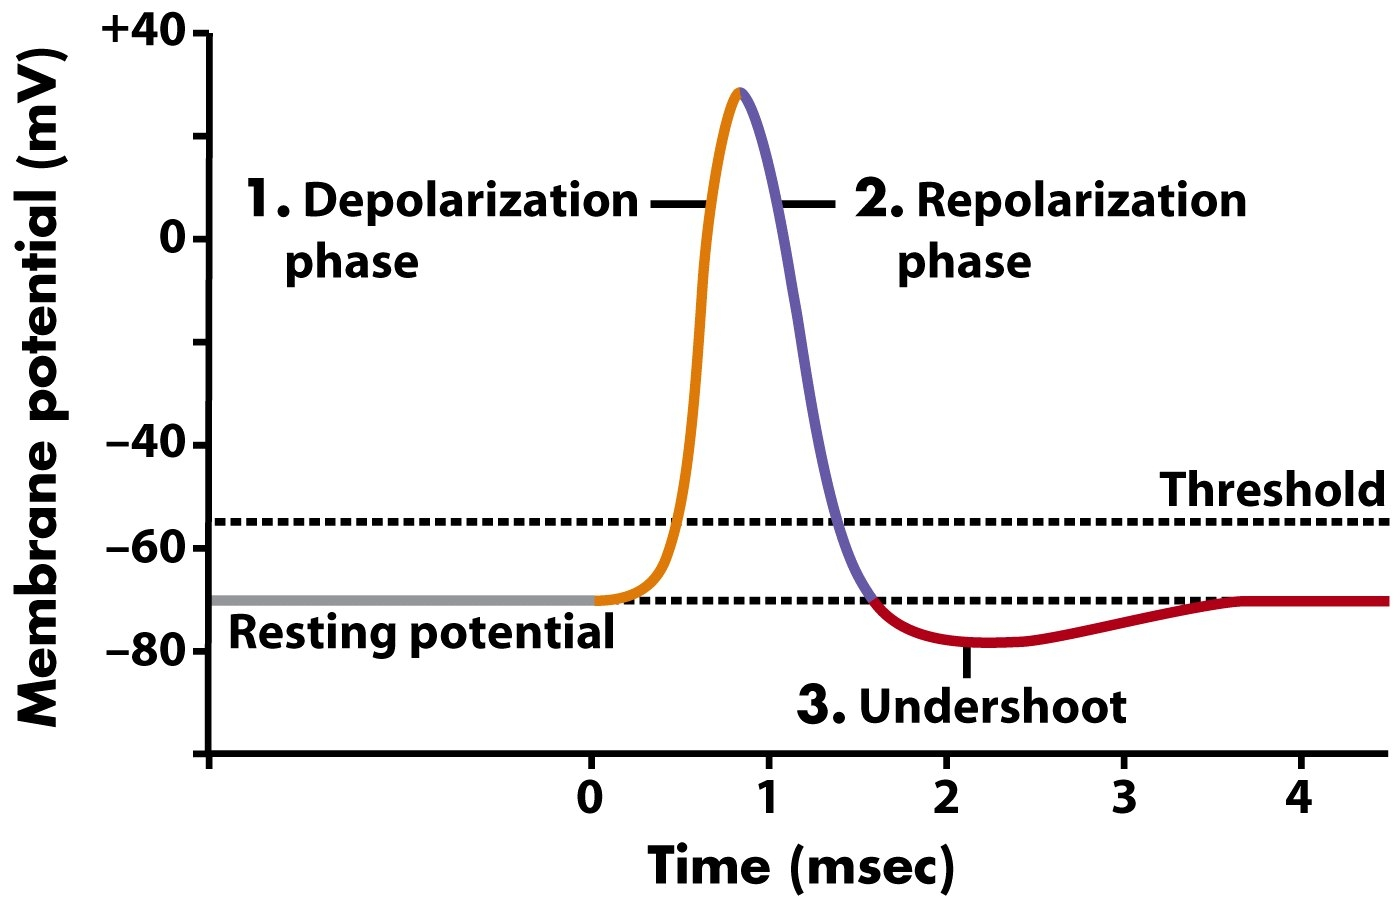
\includegraphics[scale=0.5]{action_potential}
\end{center}

\subsubsection*{Resting potiential}

Fluid on the inside of the membrane is negativly charged with respect to the
outside of the neurone. This difference is called the resting potiential.

Sodium and potassium constantly diffues through protein channels along their
electrochemical gradient. However, sodium-potassium pumps uses active transport
to move three sodium ions out of and two potassium ions into the axon,
maintaining the electrochemical gradient.

The cytoplasm of an axon contains mitochondria to supply ATP to the sodium-
potassium pumps.

\subsubsection*{Depolarisation}

When an impulse reaches a neurone, a small electrical change occurs in the cell
membrane of the axon. This has the effect of opening the gated ion channels in
the cell membrane to allow ions to flood in, making the small stretch of axon
where this impulse is occuring have a positive resting potiential.

This is an {\bf all or nothing signal}. If the action potiential is reached
inside the axon (above around $-50\milli\volt$) then the impulse is triggered.
If the action potiential isn't reached, no impulse occurs.

\subsubsection*{Action potiential}

When a patch of axon membrane depolarises, a flow of current is produced as the
electrically charged ions move. This stimulates the next patch of membrane, and
the action potiential moves along the axon.

\subsubsection*{The refactory period}

For a short time after an action potiential has passed a section of axon, the
gated ion channels remain closed, during this time, the membrane cannot be
depolarised again. This ensures that no action potientials can overlap and
action potientials can only pass in one direction.

\subsection*{Factors affecting transmission speed in neurones}

Myelinated neurones have a faster transmission speed than non-myelinated
neurones. This is because the Schwann cells that form the myelin layer prevent
the diffusion of ions. This also means that depolarisation only occurs at the
nodes of Ranvier, and the action potiential only has to jump from node to node.

Higher temperatures increase the rate of diffusion of ions, and so increases the
transmission speed.

In axons that aren't myelinated, the larger diameter of the axon, the faster the
transmission. Because of the smaller surface area to volume ratio of larger
axons, a smaller proportion of ions leak and the transmission speed is
increased.

\newpage

\section*{Transmission over synapses}

Synapses are connections between neurones. They facilitate the passage of
impulses between neurones. Here is the structure of a synapse:

\begin{center}
	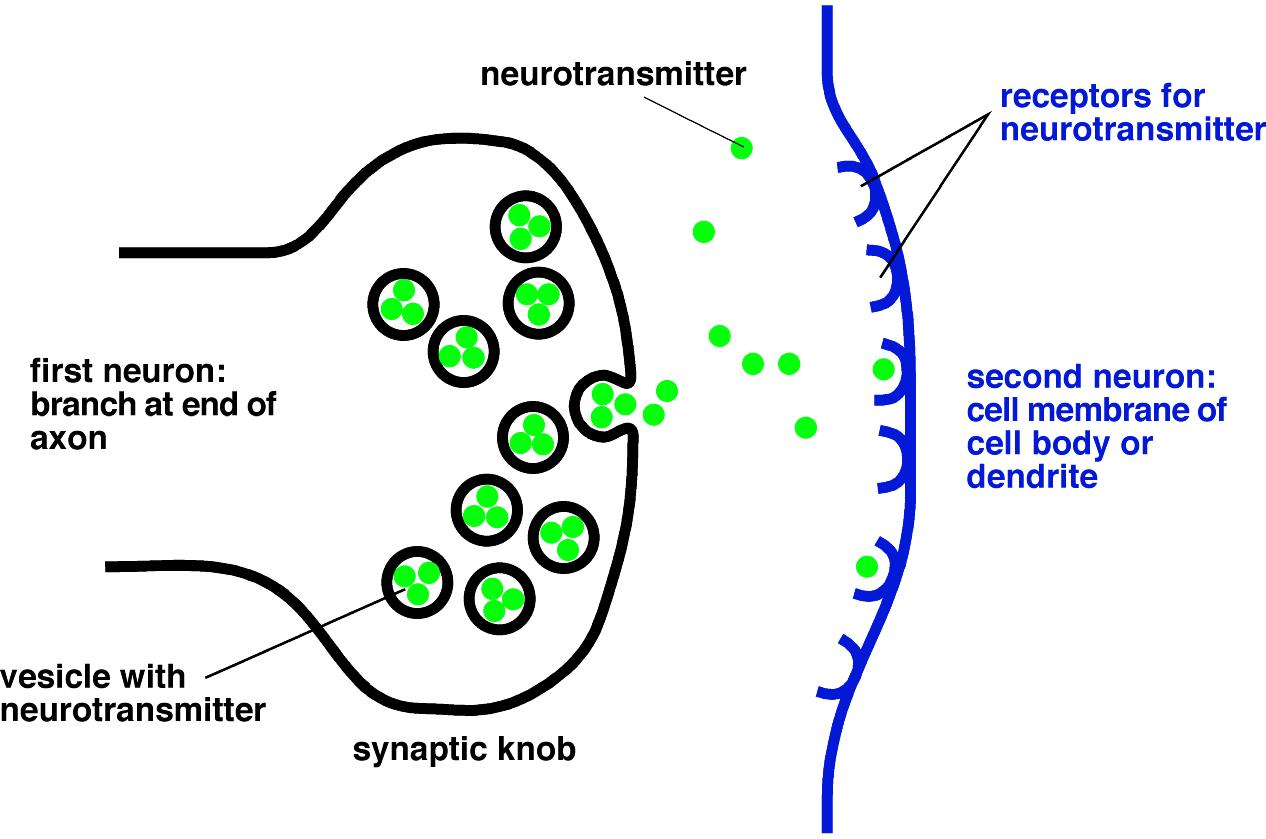
\includegraphics[scale=0.6]{synapse2}
\end{center}

Notice that the receptors are on the postsynaptic membrane, and the vesicles
containing the transmitter are on the presynaptic knob. This helps to ensure
that the impulses can only travel in one direction. Hence synapses are {\it
unidirectional}.

Synapses using acetylcholine are known as cholinergic synapses. They occur in
many parts of the nervous system, including the brain.

\subsection*{What happens when an impulse reaches a synapse?}

The stages of synaptic transmission are as follows:

\begin{enumerate}

	\item A neurotransmitter (e.g. acetlycholine) is synthesised in synaptic
	vesicles. ATP from mitochondria in the neurones powers this process.

	\item At the end of the presynaptic neurone, there are voltage gated ion
	calcium ion channels that open when an action potiential reaches the
	neurone and allow calcium ions to  diffuse into the cell.

	\item These calcium ions cause the synaptic vesicles to fuse with the cell
	membrane, releasing their contents (the neurotransmitter chemicals) by {\it
	exocytosis}.

	\item The neurotransmitter then diffuses across the synaptic cleft.

	\item The neurotransmitter binds to the neuroreceptors in the postsynaptic
	membrane, which causes sodium ion channels to open, making the membrane
	more permiable to that ion.

	\item This causes a depolarisation of the postsynaptic cell membrane, which
	may initiate an action potiential.

	\item The neurotransmitter is then broken down by an enzyme (e.g.
	acetylcholinesterase breaks down acetylcholine). The presynaptic neurone
	then absorbs the products of this breakdown (by endocytosis) and use them
	to re-synthesise more neurotransmitter using ATP from mitochondria.

\end{enumerate}

\subsection*{Factors affecting synapse transmission}

There are many chemicals that can have an effect on synapse transmission. Some
drugs are able to mimic the neuroreceptor (e.g. nicotine), stimulate
neuroreceptor release (e.g. caffine), block neutoreceptor channels (e.g.
curare), prevent neurotransmitter release (e.g. botulin toxin) or inhibit the
enzyme that breaks down the neuroreceptor (e.g. organophosphates).

\subsection*{Summation}

Summation referes to how different impulses can combine at one nerve cell to
produce another impulse. There are two types of summation, temporal and spatial.

\subsubsection*{Temporal summation}

When two or more impulses arrive in quick succession at a synapse, the membrane
potiential may not have chance to reset back to the resting potiential,
increasing the chance that an action potiential will be reached. This only
occurs in neurones with one presynaptic neurone and one postsynaptic neurone.

\subsubsection*{Spacial summation}

In spatial summation, several presynaptic neurones converge at a synapse with a
single post synaptic neurone. The sum of their membrane potentials may or may
not trigger an action potiential. Some of the presynaptic neurones may be
inhibitory.

\end{document}